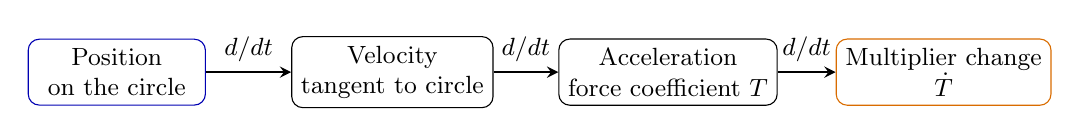
\begin{tikzpicture}[>=stealth,box/.style={draw,rounded corners,align=center,font=\small,minimum width=2.25cm,minimum height=.8cm}]
\node[box,draw=blue!70!black](a)at(0,0){Position\\on the circle};
\node[box](b)at(3.5,0){Velocity\\tangent to circle};
\node[box](c)at(7,0){Acceleration\\force coefficient $T$};
\node[box,draw=orange!85!black](d)at(10.5,0){Multiplier change\\$\dot T$};
\draw[->,thick](a)--node[above,font=\small]{$d/dt$}(b);
\draw[->,thick](b)--node[above,font=\small]{$d/dt$}(c);
\draw[->,thick](c)--node[above,font=\small]{$d/dt$}(d);
\end{tikzpicture}
